\documentclass[a4paper, 14pt]{extarticle}
\usepackage[russian]{babel}
\usepackage[T1]{fontenc}
\usepackage{fontspec}
\usepackage{indentfirst}
\usepackage{enumitem}
\usepackage{graphicx}
\usepackage[
  left=20mm,
  right=10mm,
  top=20mm,
  bottom=20mm
]{geometry}
\usepackage{parskip}
\usepackage{titlesec}
\usepackage{xurl}
\usepackage{hyperref}
\usepackage{float}
\usepackage[
  figurename=Рисунок,
  labelsep=endash,
]{caption}
\usepackage[outputdir=build, newfloat]{minted}

\hypersetup{
  colorlinks=true,
  linkcolor=black,
  filecolor=blue,
  urlcolor=blue,
}

\renewcommand*{\labelitemi}{---}
\setmainfont{Times New Roman}
\setmonofont{JetBrains Mono}[
  SizeFeatures={Size=11},
]

\newenvironment{code}{\captionsetup{type=listing}}{}
\SetupFloatingEnvironment{listing}{name=Листинг}

\setminted{
  fontsize=\footnotesize,
  frame=lines,
  framesep=2mm,
}

\setlength{\parskip}{6pt}

\setlength{\parindent}{1cm}
\setlist[itemize]{itemsep=0em,topsep=0em,parsep=0em,partopsep=0em,leftmargin=2.0cm}
\setlist[enumerate]{itemsep=0em,topsep=0em,parsep=0em,partopsep=0em,leftmargin=2.0cm}

\renewcommand{\thesection}{\arabic{section}.}
\renewcommand{\thesubsection}{\thesection\arabic{subsection}.}
\renewcommand{\thesubsubsection}{\thesubsection\arabic{subsubsection}.}

\titleformat{\section}{\normalfont\bfseries}{\thesection}{0.5em}{}
\titleformat{\subsection}{\normalfont\bfseries}{\thesubsection}{0.5em}{}

\titleformat*{\section}{\normalfont\bfseries}
\titleformat*{\subsection}{\normalfont\bfseries}

\linespread{1.5}
\renewcommand{\baselinestretch}{1.5}
\begin{document}

\begin{titlepage}
  \vspace{0pt plus2fill}
  \noindent

  \vspace{0pt plus6fill}
  \begin{center}
    Санкт-Петербургский национальный исследовательский университет
    информационных технологий, механики и оптики

    \vspace{0pt plus3fill}

    Факультет инфокоммуникационных технологий

    Направление подготовки 11.03.02

    \vspace{0pt plus2fill}

    Практическая работа №1

    <<Консольные утилиты настройки сетевых \\ компонентов в ОС Windows>>

  \end{center}

  \vspace{0pt plus9fill}
  \begin{flushright}
    Выполнил: \\
    Швалов Даниил Андреевич

    Группа: К33211

    Проверил: \\
    Харитонов Антон
  \end{flushright}

  \vspace{0pt plus2fill}
  \begin{center}
    Санкт-Петербург

    2023
  \end{center}
\end{titlepage}

\setcounter{page}{2}

\section{Введение}

\textbf{Цель работы}: получить практические навыки по конфигурированию сети в
операционных системах Microsoft Windows, ознакомится с утилитами командной
строки, предназначенными для диагностики и настройки сети, разработать
исполняемые файлы, конфигурирующие сетевой интерфейс по заданным параметрам,
ознакомиться с форматом записи пути до сетевого ресурса UNC.

\section{Ход работы}

\subsection{Исследование сетевых компонентов}

На рис. \ref{fig:ethernet-properties} изображены сетевые компоненты,
используемые в системе. Рассмотрим некоторые из них:
\begin{itemize}
  \item Клиент для сетей Microsoft (Client for Microsoft Networks) --- это
  программный компонент, который позволяет компьютеру выполнять в сети
  Microsoft доступ к таким ресурсам, как файловые службы, службы печати и
  другим общим сетевым ресурсам.

  \item Служба доступа к файлам и принтерам Microsoft (File and Printer Sharing
  for Microsoft Networks) --- это служба, которая дополняет службу
  <<Клиент для сетей Microsoft>>. Она позволяет компьютерам сети
  выполнять доступ к файлам и принтерам, которые настроил пользователь
  для разделяемого доступа.

  \item Протокол TCP/IP --- это компонент, который обеспечивает работу стека
  TCP/IP в Windows.
\end{itemize}

\begin{figure}[H]
  \centering
  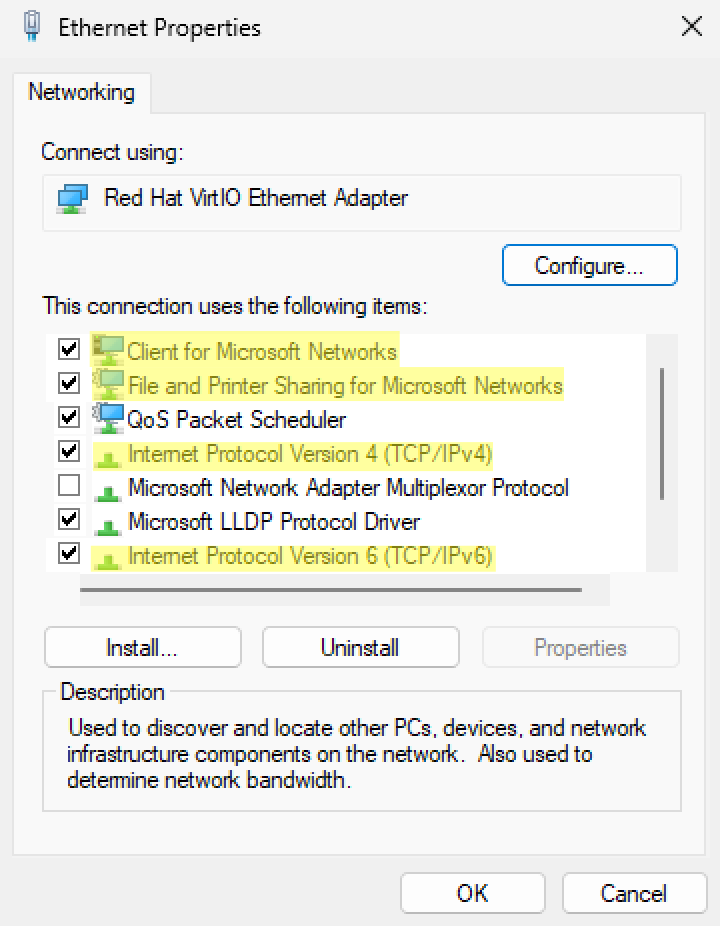
\includegraphics[width=0.5\textwidth]{images/ethernet-properties.png}
  \caption{Сетевые компоненты}
  \label{fig:ethernet-properties}
\end{figure}

\subsection{Отключение доступа к ресурсам компьютера}

SMB (Server Message Block) — сетевой протокол прикладного уровня для удалённого
доступа к файлам, принтерам и другим сетевым ресурсам, а также для
межпроцессного взаимодействия. Протокол SMB используется в сетевом компоненте
<<Служба доступа к файлам и принтерам Microsoft>>. Поэтому, чтобы внешние
пользователи не могли получить доступ к ресурсам компьютера по протоколу SMB,
необходимо отключить компонент <<Служба доступа к файлам и принтерам
Microsoft>>.

\subsection{Утилита ping}

Утилита \texttt{ping} проверяет подключение на уровне IP-адреса к другому
компьютеру, отправляя сообщения запроса на эхо-запрос по протоколу ICMP. При
использовании без параметров эта команда отображает содержимое справки.

При использовании \texttt{ping} только с адресом, без дополнительных флагов,
будет выполнено 4 запроса, после чего программа завершится (см. рис.
\ref{fig:ping-default}).

\begin{figure}[H]
  \centering
  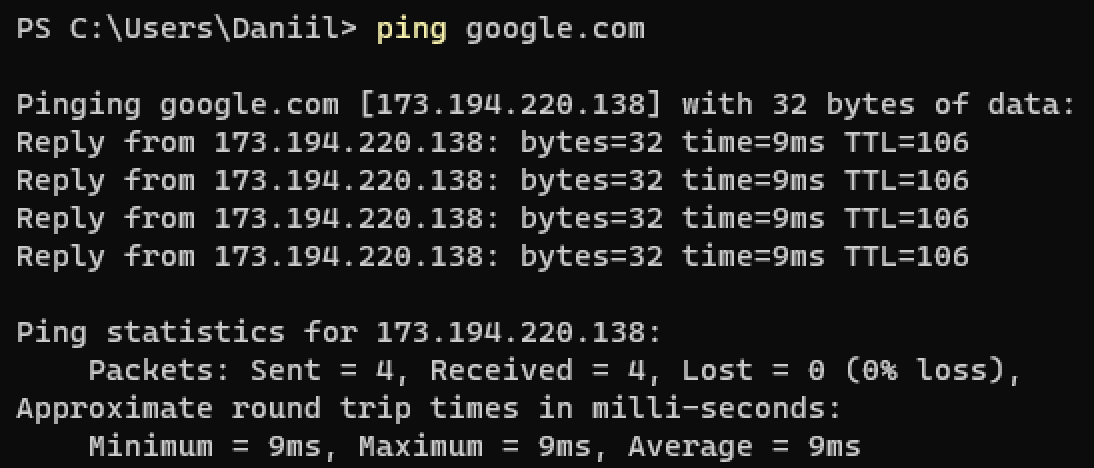
\includegraphics[width=0.9\textwidth]{images/ping/default.png}
  \caption{Использование \texttt{ping} без дополнительных параметров}
  \label{fig:ping-default}
\end{figure}

Параметр \texttt{-t} используется для проверки доступности до тех пор, пока
пользователь не прервет выполнение программы, например, с помощью
\texttt{CTRL-C} (см. рис. \ref{fig:ping-infinity}).

\begin{figure}[H]
  \centering
  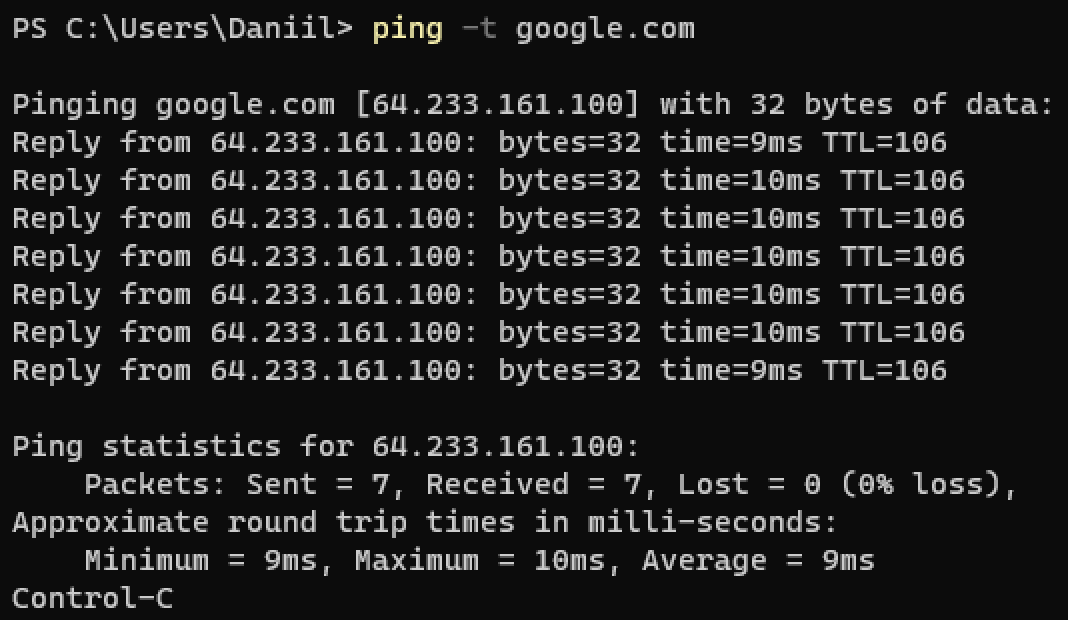
\includegraphics[width=0.9\textwidth]{images/ping/infinity.png}
  \caption{Использование \texttt{ping} с параметром \texttt{-t}}
  \label{fig:ping-infinity}
\end{figure}

Параметр \texttt{-n} используется для указания количества ICMP-запросов (см.
рис. \ref{fig:ping-n}).

\begin{figure}[H]
  \centering
  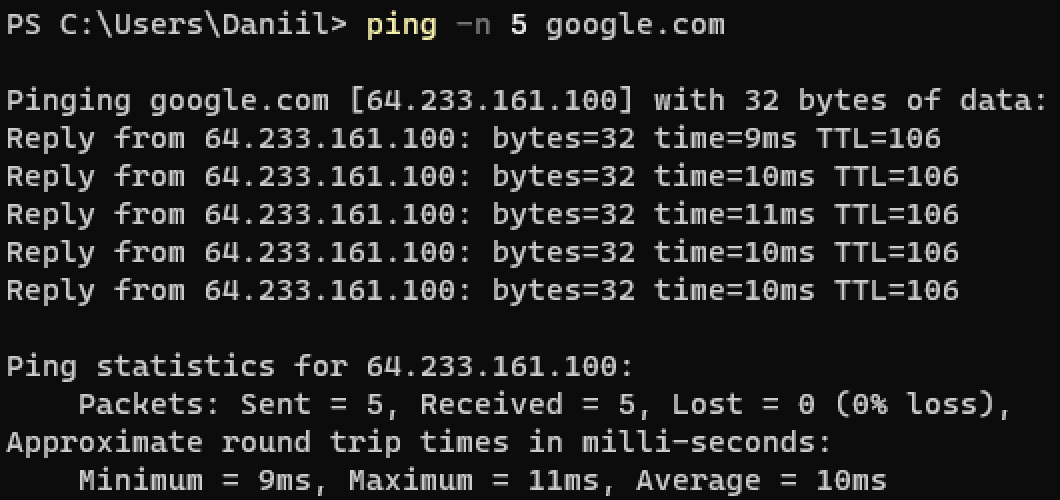
\includegraphics[width=0.9\textwidth]{images/ping/n.png}
  \caption{Использование \texttt{ping} с параметром \texttt{-n}}
  \label{fig:ping-n}
\end{figure}

Параметр \texttt{-l} используется для указания размера отправляемого пакета
(см. рис. \ref{fig:ping-size}).

\begin{figure}[H]
  \centering
  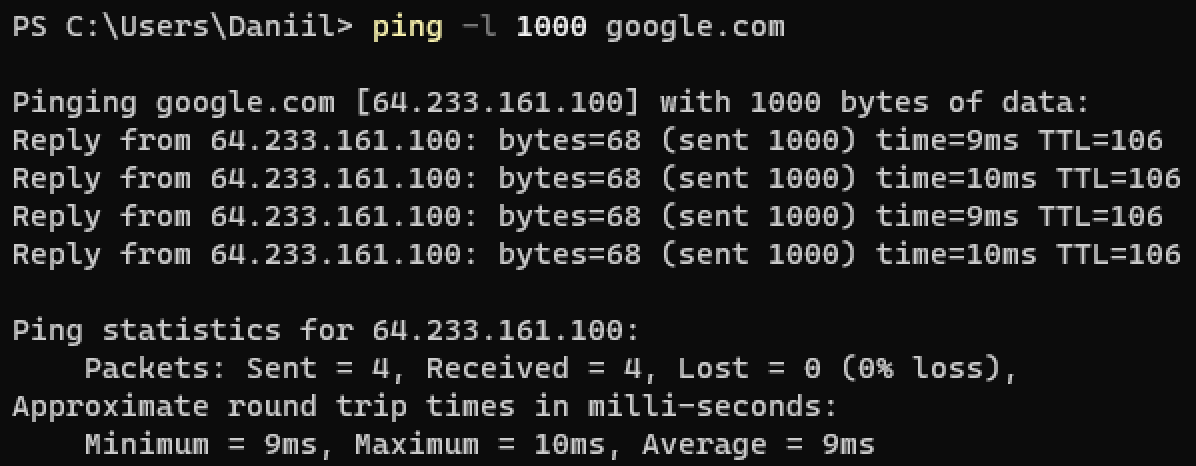
\includegraphics[width=0.9\textwidth]{images/ping/size.png}
  \caption{Использование \texttt{ping} с параметром \texttt{-l}}
  \label{fig:ping-size}
\end{figure}

Для перенаправления вывода утилиты \texttt{ping} и сохранения вывода в файл
используется символ \texttt{>} (см. рис \ref{fig:ping-file}).

\begin{figure}[H]
  \centering
  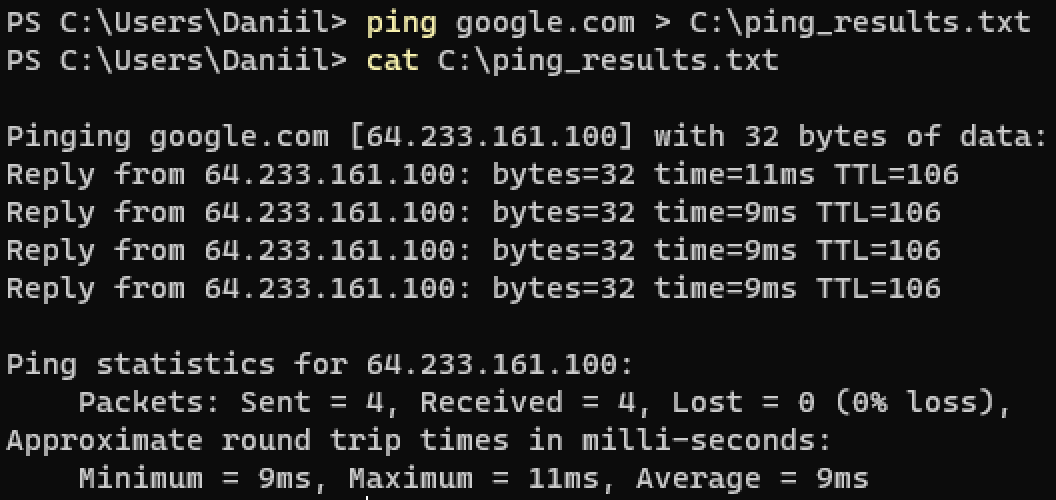
\includegraphics[width=0.9\textwidth]{images/ping/file.png}
  \caption{Перенаправление вывода \texttt{ping} в файл}
  \label{fig:ping-file}
\end{figure}

\subsection{Утилита tracert}

Утилита \texttt{tracert} используется для отслеживания маршрута, который
проходит от сетевой пакет компьютера до удаленного хоста.

При использовании \texttt{tracert} только с адресом, без дополнительных флагов,
сделает максимум 30 прыжков (или меньше, если путь от компьютера до удаленного
хоста содержит меньше узлов), после чего программа завершится (см. рис.
\ref{fig:tracert-default}).

\begin{figure}[H]
  \centering
  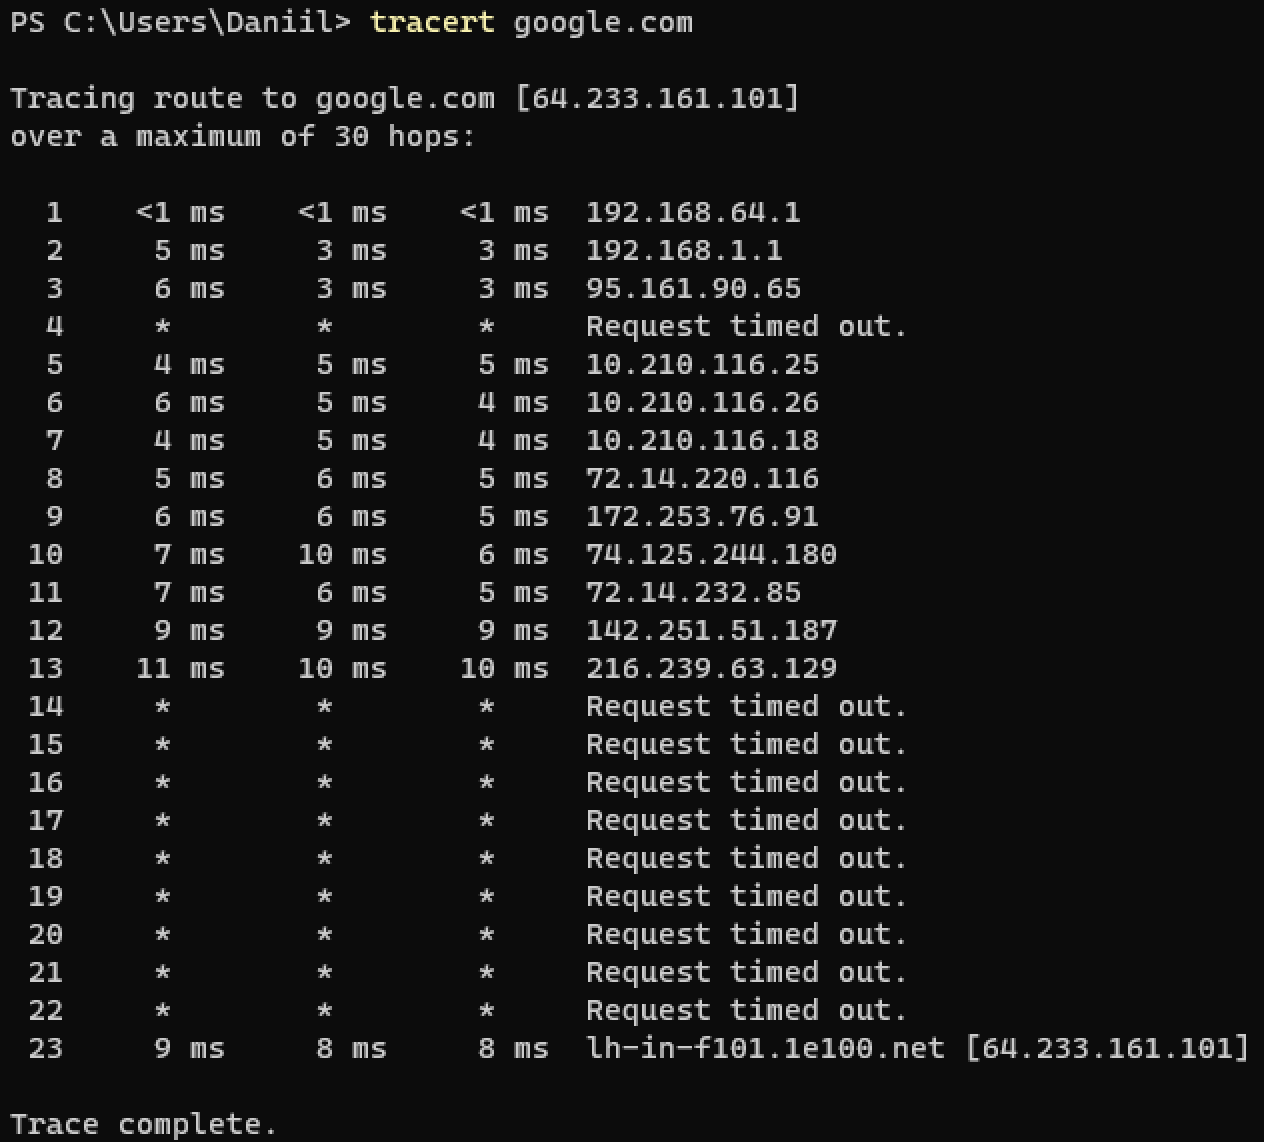
\includegraphics[width=0.9\textwidth]{images/tracert/default.png}
  \caption{Использование \texttt{tracert} без дополнительных опций}
  \label{fig:tracert-default}
\end{figure}

Параметр \texttt{-h} используется для указания максимального количества
прыжком, после которого программа завершит свою работу (см. рис.
\ref{fig:tracert-hops}).

\begin{figure}[H]
  \centering
  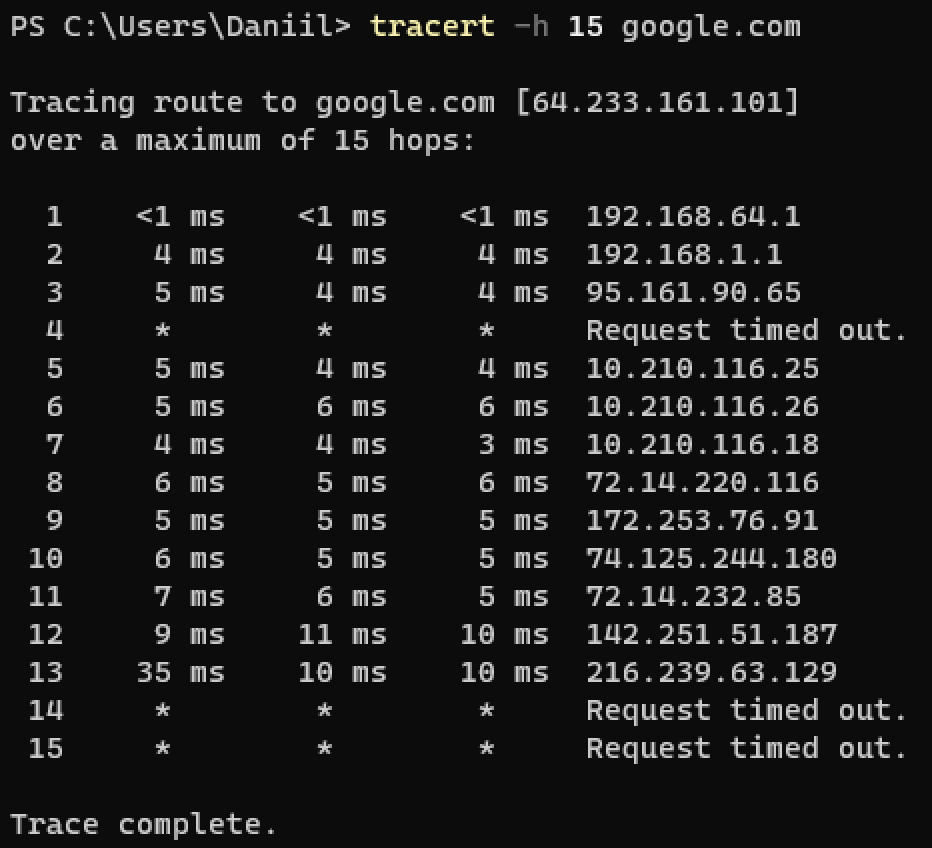
\includegraphics[width=0.7\textwidth]{images/tracert/hops.png}
  \caption{Использование \texttt{tracert} с параметром \texttt{-h}}
  \label{fig:tracert-hops}
\end{figure}

Параметр \texttt{-w} используется для указания максимального времени ожидания
ответа от узла на ICMP-запрос. При истечении этого времени программа переходит
к следующему по пути следования пакета хосту (см. рис.
\ref{fig:tracert-timeout}).

\begin{figure}[H]
  \centering
  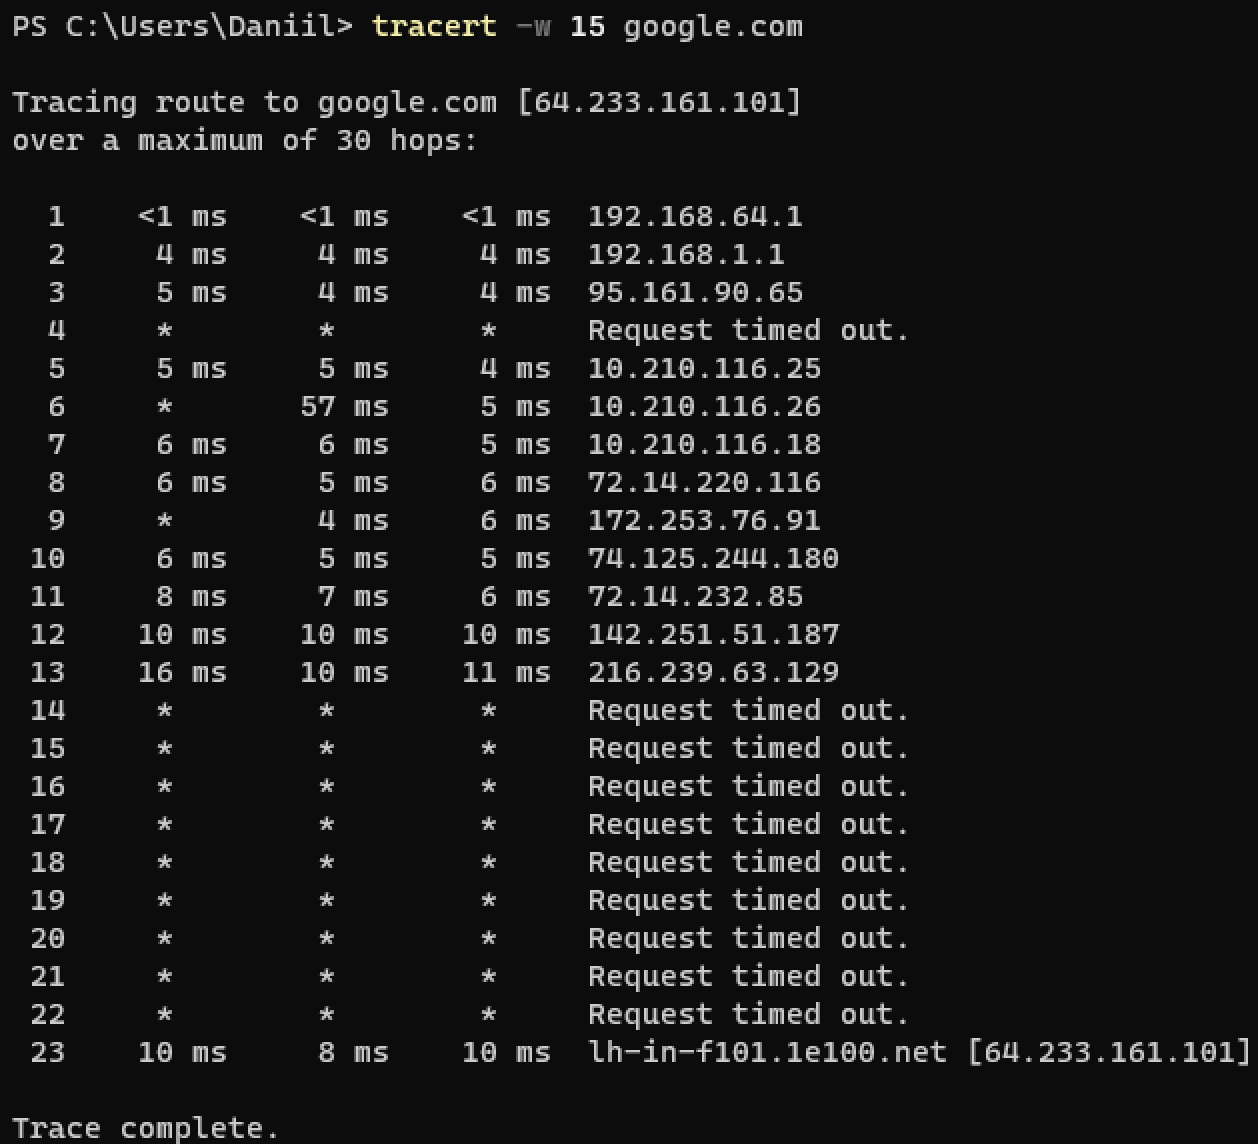
\includegraphics[width=0.9\textwidth]{images/tracert/timeout.png}
  \caption{Использование \texttt{tracert} с параметром \texttt{-w}}
  \label{fig:tracert-timeout}
\end{figure}

\subsection{Утилита ipconfig}

Утилита \texttt{ipconfig} используется для получения таких параметров как
IP-адрес компьютера, маска подсети, IP-адрес шлюза, а также для обновления и
изменения настроек DHCP и DNS.

При использовании \texttt{ipconfig} без параметров пользователю будут
отображены основные сетевые настройки всех сетевых адаптеров, присутствующих в
системе (см. рис. \ref{fig:ipconfig-default}).

\begin{figure}[H]
  \centering
  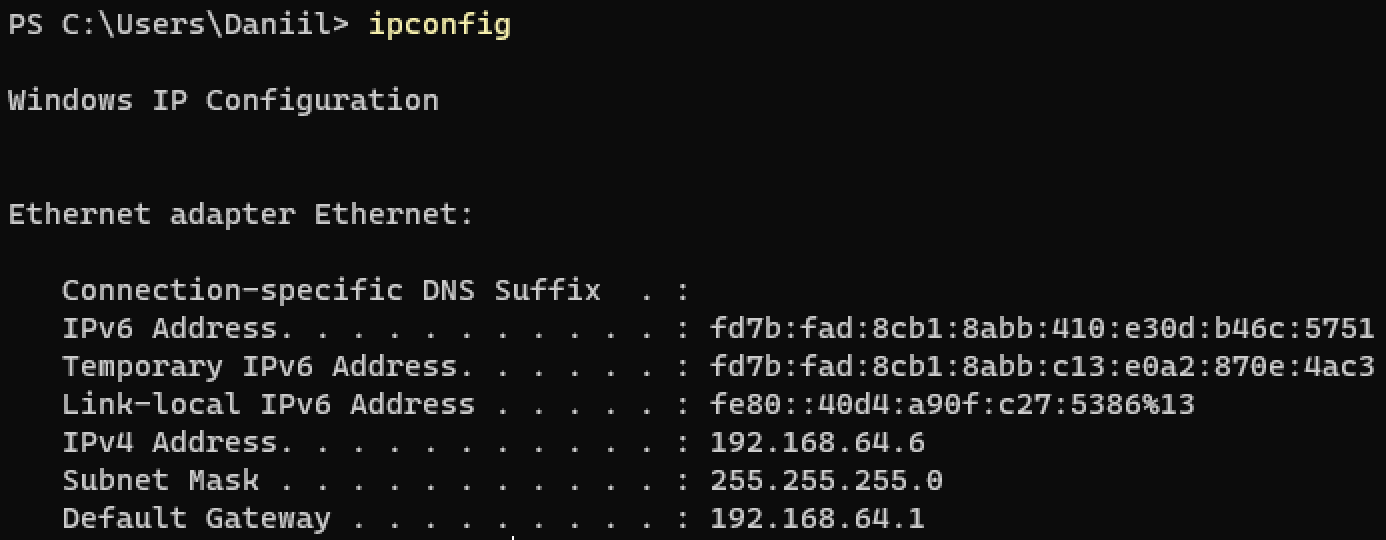
\includegraphics[width=0.9\textwidth]{images/ipconfig/default.png}
  \caption{Использование \texttt{ipconfig} без дополнительных параметров}
  \label{fig:ipconfig-default}
\end{figure}

Команда \texttt{ipconfig /all} выводит более подробную информацию о настройках
сетевых адаптеров, например, адреса DNS серверов, адрес DHCP сервера и т. д.
(см. рис. \ref{fig:ipconfig-all}).

\begin{figure}[H]
  \centering
  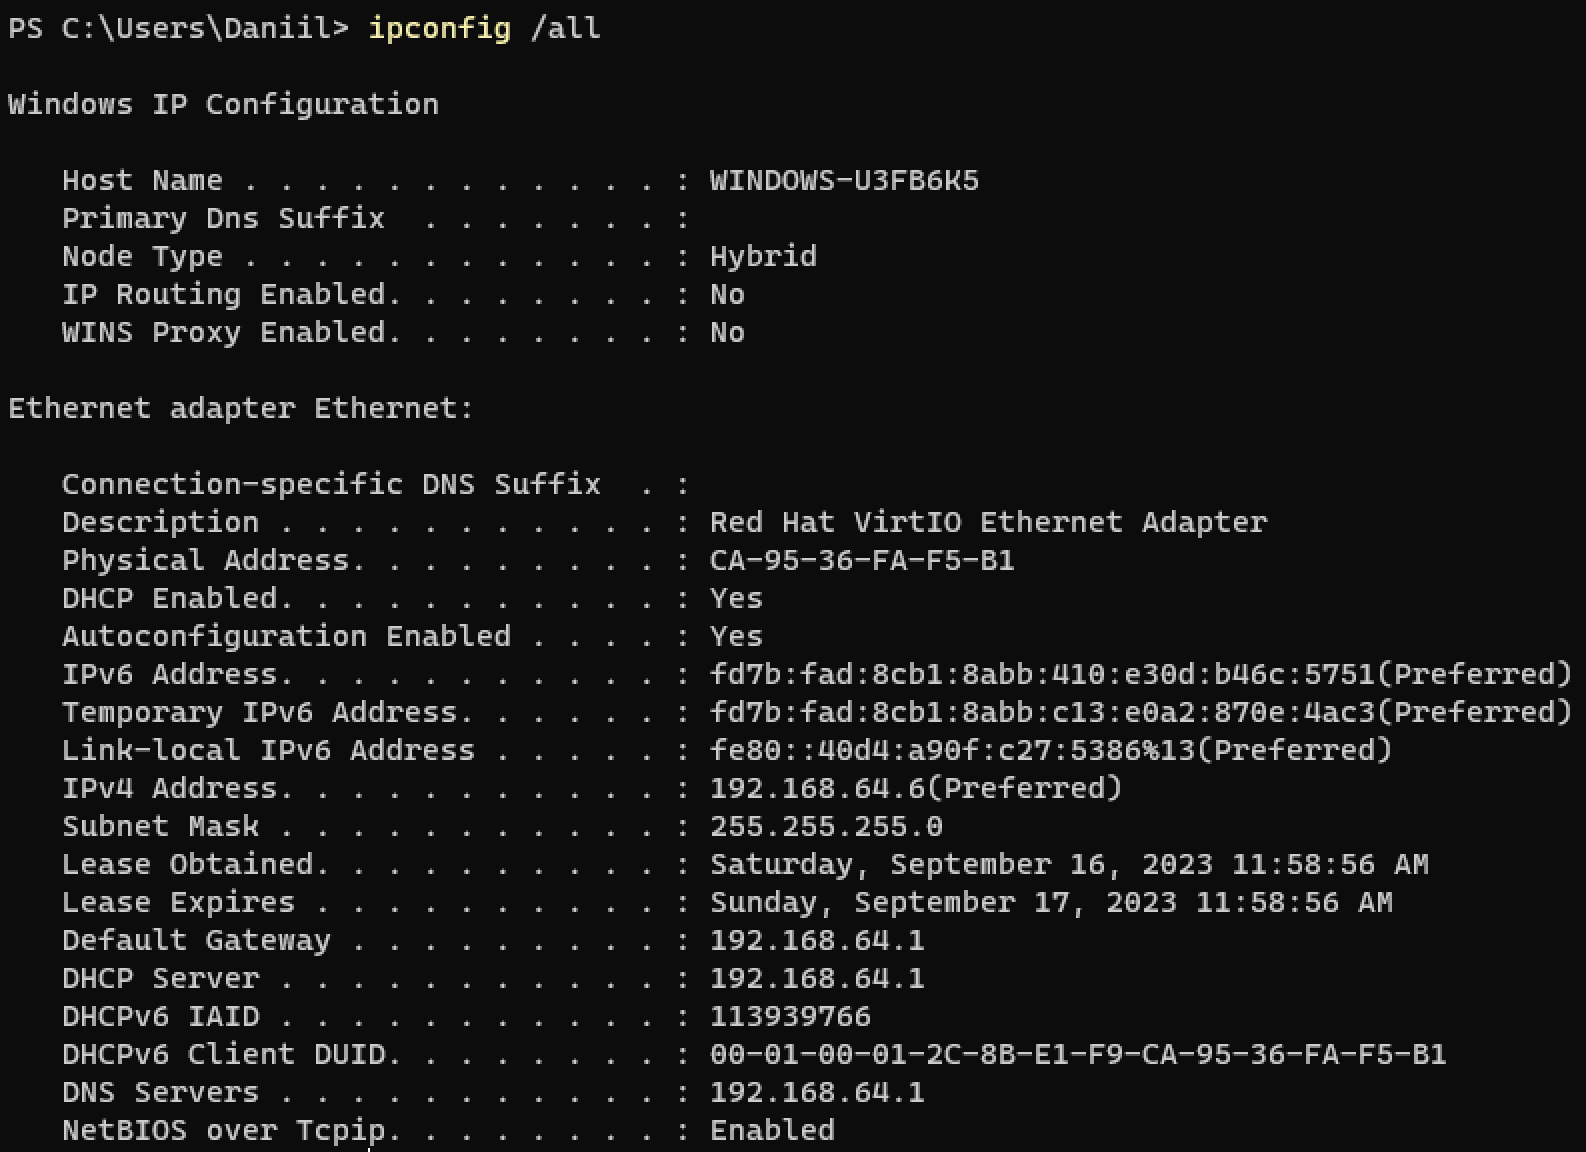
\includegraphics[width=0.9\textwidth]{images/ipconfig/all.png}
  \caption{Использование \texttt{ipconfig} с параметром \texttt{/all}}
  \label{fig:ipconfig-all}
\end{figure}

Для того, чтобы освободить IP-адрес, выданный DHCP сервером, используется
команда \texttt{ipconfig /release} (см. рис. \ref{fig:ipconfig-release}).

\begin{figure}[H]
  \centering
  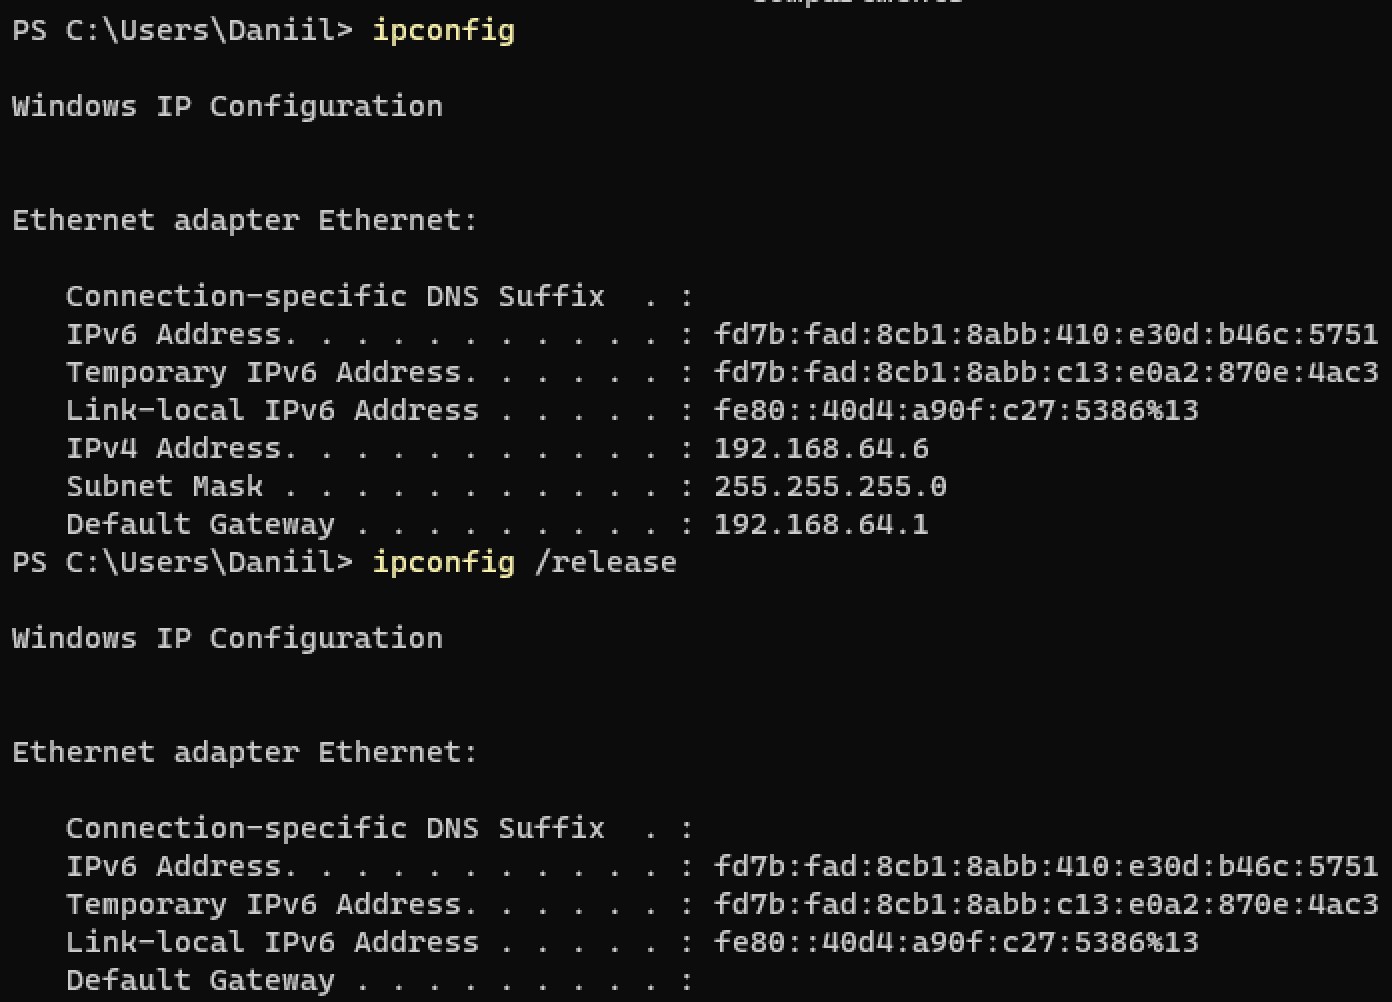
\includegraphics[width=0.9\textwidth]{images/ipconfig/release.png}
  \caption{Использование \texttt{ipconfig} с параметром \texttt{/release}}
  \label{fig:ipconfig-release}
\end{figure}

Для получения нового IP-адреса от DHCP сервера используется команда
\texttt{ipconfig /renew} (см. рис. \ref{fig:ipconfig-renew}).

\begin{figure}[H]
  \centering
  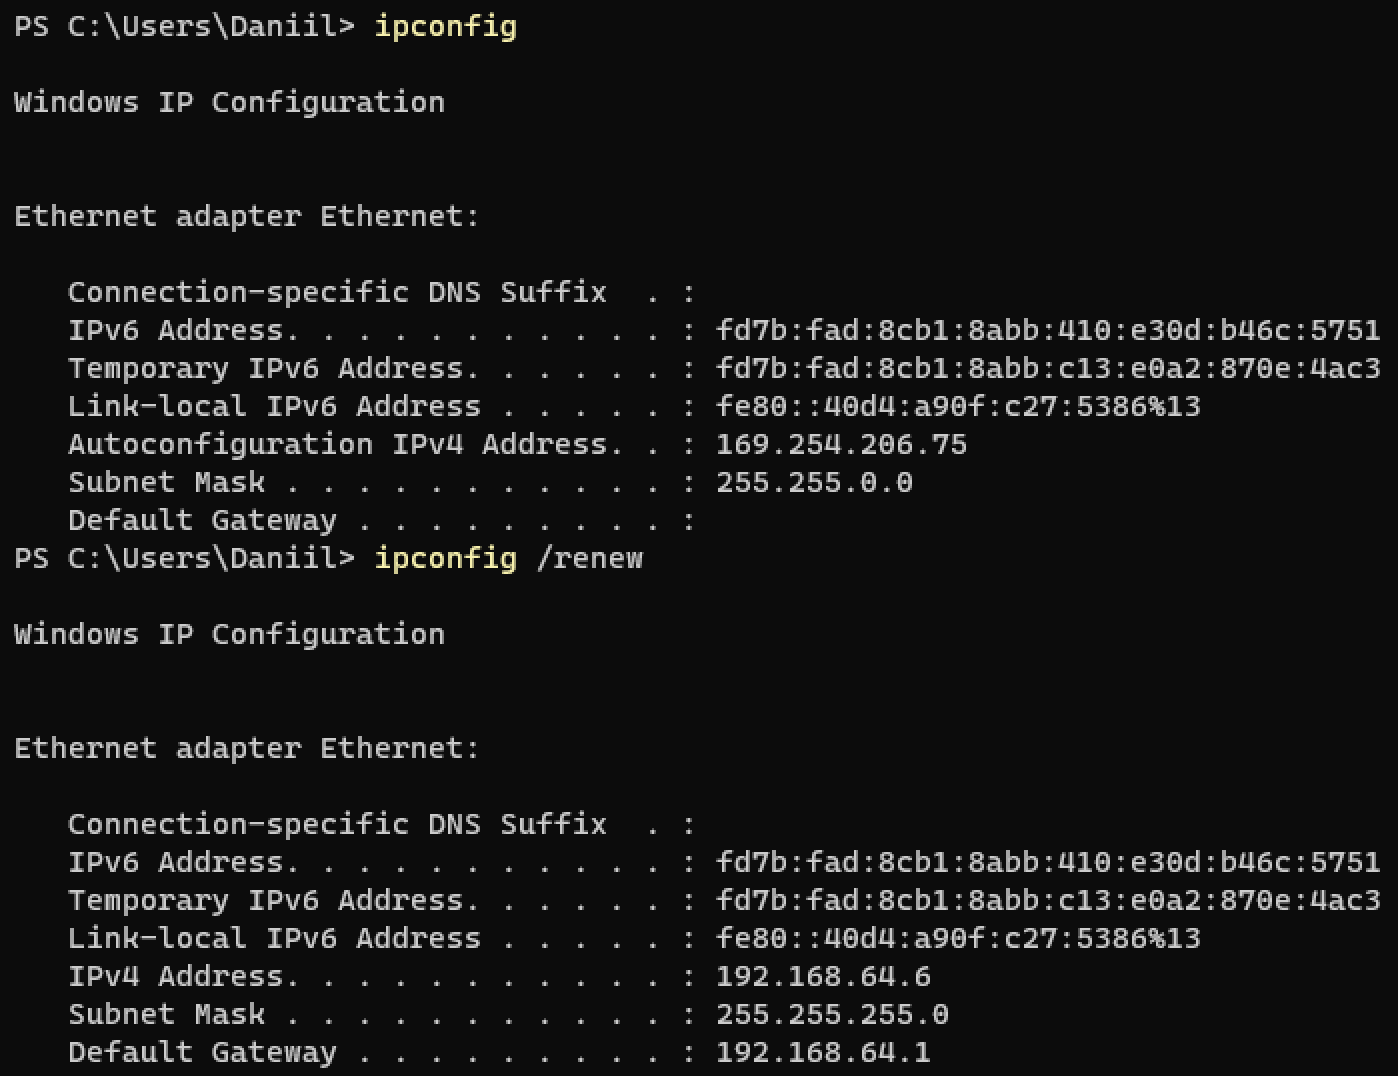
\includegraphics[width=0.9\textwidth]{images/ipconfig/renew.png}
  \caption{Использование \texttt{ipconfig} с параметром \texttt{/renew}}
  \label{fig:ipconfig-renew}
\end{figure}

Для получения содержимого кэша DNS клиента используется команда
\texttt{ipconfig /displaydns} (см. рис. \ref{fig:ipconfig-displaydns}).

\begin{figure}[H]
  \centering
  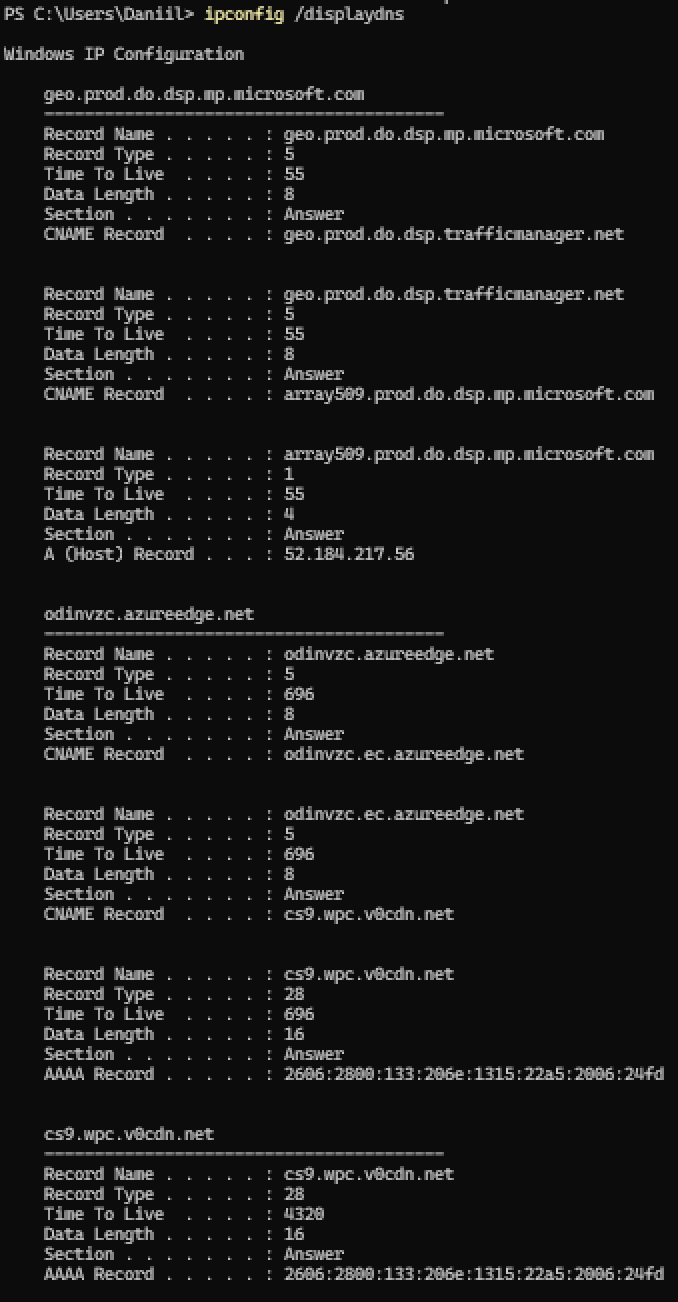
\includegraphics[width=0.7\textwidth]{images/ipconfig/displaydns.png}
  \caption{Использование \texttt{ipconfig} с параметром \texttt{/displaydns}}
  \label{fig:ipconfig-displaydns}
\end{figure}

Для обновления всех хранимых DNS-имен используется команда \texttt{ipconfig
  /registerdns} (см. рис. \ref{fig:ipconfig-registerdns}).

\begin{figure}[H]
  \centering
  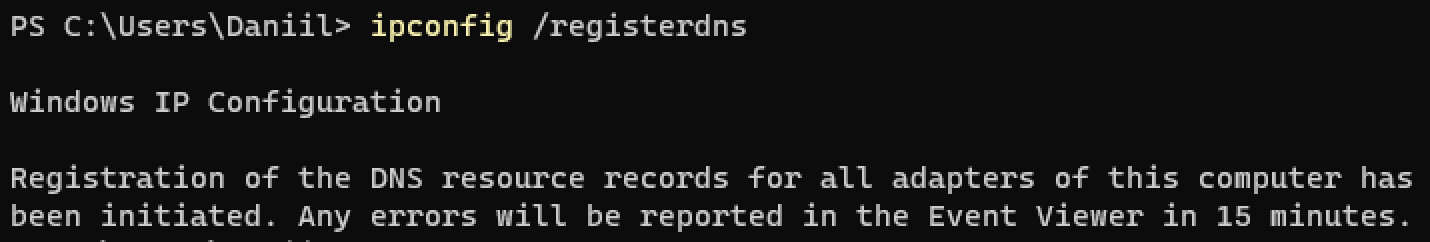
\includegraphics[width=0.9\textwidth]{images/ipconfig/registerdns.png}
  \caption{Использование \texttt{ipconfig} с параметром \texttt{/registerdns}}
  \label{fig:ipconfig-registerdns}
\end{figure}

Для сбора кэша DNS клиента используется команда \texttt{ipconfig /flushdns}
(см. рис. \ref{fig:ipconfig-flushdns}).

\begin{figure}[H]
  \centering
  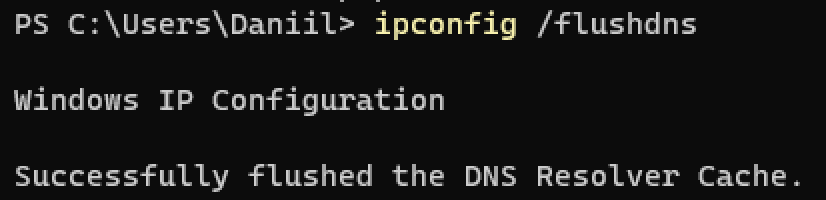
\includegraphics[width=0.7\textwidth]{images/ipconfig/flushdns.png}
  \caption{Использование \texttt{ipconfig} с параметром \texttt{/flushdns}}
  \label{fig:ipconfig-flushdns}
\end{figure}

\subsection{Утилита net}

\texttt{net.exe} --- это утилита управления сетевой конфигурацией, которая
позволяет подключать и отключать сетевые диски, запускать и останавливать
системные службы, добавлять и удалять пользователей, управлять совместно
используемыми ресурсами, устанавливать системное время, отображать
статистические и справочные данные об использовании ресурсов.

Команда \texttt{net use} подключает или отключает компьютер к общему ресурсу.
Когда команда используется без параметров, выводится список подключений данного
компьютера. При использовании команды без аргументов выводится список
существующих подключений (см. рис. \ref{fig:net-use}). При указании конкретного
подключения в качестве аргумента команды (например, \texttt{net use X:}) будет
выведена информация об этом подключении.

\begin{figure}[H]
  \centering
  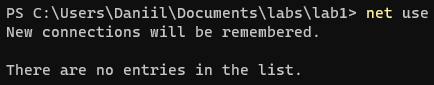
\includegraphics[width=0.7\textwidth]{images/net/use.png}
  \caption{Список существующих подключений}
  \label{fig:net-use}
\end{figure}

Команда \texttt{net view} отображает список общих ресурсов компьютера. При
использовании без параметров отображается список всех компьютеров в текущем
домене или рабочей группе (см. рис. \ref{fig:net-view}). При указании
конкретного компьютера в качестве аргумента команды (например, \texttt{net view
  \textbackslash\textbackslash WINDOWS-U3FB6K5}) будет выведена информация о
общих ресурсах устройства (см. рис. \ref{fig:net-view-computer}).

\begin{figure}[H]
  \centering
  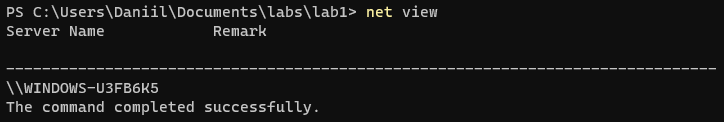
\includegraphics[width=0.9\textwidth]{images/net/view.png}
  \caption{Список общих ресурсов компьютера}
  \label{fig:net-view}
\end{figure}

\begin{figure}[H]
  \centering
  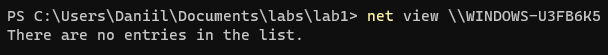
\includegraphics[width=0.9\textwidth]{images/net/view-computer.png}
  \caption{Список общих ресурсов устройства}
  \label{fig:net-view-computer}
\end{figure}

Команды \texttt{net start} и \texttt{net stop} используется для запуска и
остановки системных служб Windows соответственно. В качестве аргумента эти
команды принимают название службы, которую нужно запустить или остановить.
Пример использования команды показан на рис. \ref{fig:net-start-stop}.

\begin{figure}[H]
  \centering
  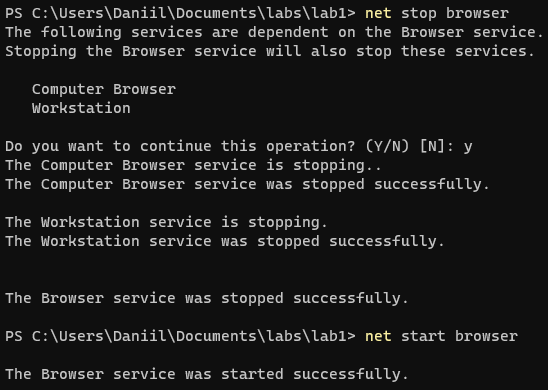
\includegraphics[width=0.8\textwidth]{images/net/start-stop.png}
  \caption{Остановка и запуск службы Computer Browser}
  \label{fig:net-start-stop}
\end{figure}

Команда \texttt{net share} разрешает использовать ресурсы компьютера другим
пользователям сети. Когда команда используется без параметров, выводится
информация о всех общих ресурсах компьютера (см. рис. \ref{fig:net-share}). При
передаче названия ресурса в качестве аргумента будет отображаться информация об
этом ресурсе (см. рис. \ref{fig:net-share-disk}).

\begin{figure}[H]
  \centering
  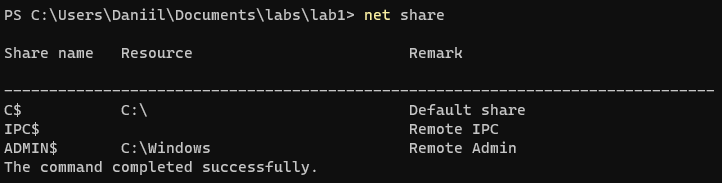
\includegraphics[width=0.9\textwidth]{images/net/share.png}
  \caption{Просмотр доступных ресурсов}
  \label{fig:net-share}
\end{figure}

\begin{figure}[H]
  \centering
  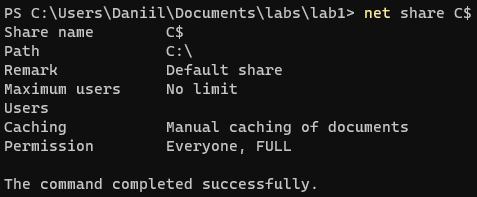
\includegraphics[width=0.9\textwidth]{images/net/share-disk.png}
  \caption{Просмотр информации о диске}
  \label{fig:net-share-disk}
\end{figure}

Команда \texttt{net config} отображает информацию о настройке служб рабочей
станции или службы сервера. Когда эта команда используется без указания
параметра \texttt{server} или \texttt{workstation}, выводится список
настраиваемых служб (см. рис. \ref{fig:net-config}). При выполнении команды
\texttt{net config server} выводится информация о настройке службы сервера, а
при выполнении \texttt{net config workstation} --- о настройке службы рабочей
станции. (см. рис. \ref{fig:net-config-server} и
\ref{fig:net-config-workstation}).

\begin{figure}[H]
  \centering
  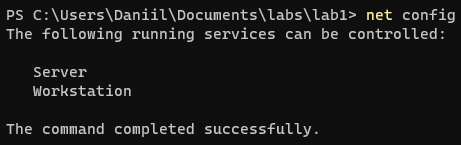
\includegraphics[width=0.7\textwidth]{images/net/config.png}
  \caption{Просмотр информации о настройке служб}
  \label{fig:net-config}
\end{figure}

\begin{figure}[H]
  \centering
  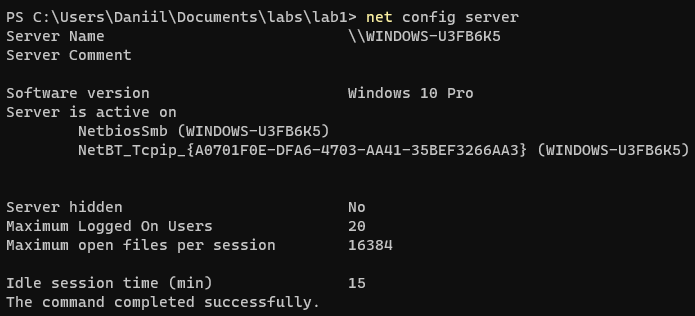
\includegraphics[width=0.9\textwidth]{images/net/config-server.png}
  \caption{Просмотр информации о настройке служб сервера}
  \label{fig:net-config-server}
\end{figure}

\begin{figure}[H]
  \centering
  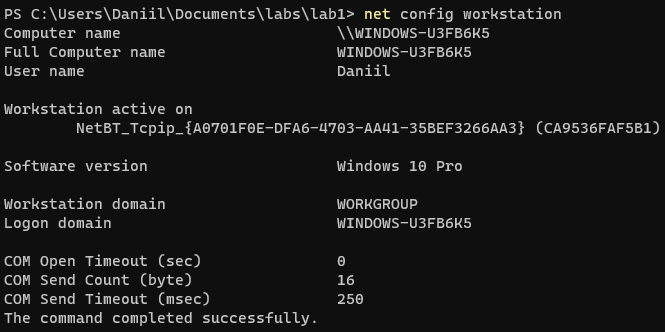
\includegraphics[width=0.9\textwidth]{images/net/config-workstation.png}
  \caption{Просмотр информации о настройке служб рабочей станции}
  \label{fig:net-config-workstation}
\end{figure}

Команда \texttt{net session} выводит их информацию о всех текущих сеансах связи
с другими компьютерами (см. рис. \ref{fig:net-session}).

\begin{figure}[H]
  \centering
  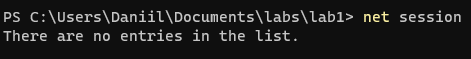
\includegraphics[width=0.7\textwidth]{images/net/session.png}
  \caption{Просмотр информации о сеансах связи}
  \label{fig:net-session}
\end{figure}

Команда \texttt{net user} используется для создания и изменения учетных записей
пользователей на компьютерах. При выполнении команды без параметров
отображается список учетных записей пользователей данного компьютера (см. рис.
\ref{fig:net-user}).

\begin{figure}[H]
  \centering
  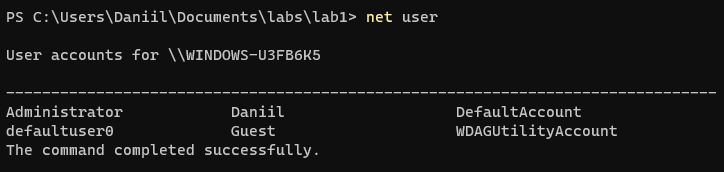
\includegraphics[width=0.9\textwidth]{images/net/user.png}
  \caption{Просмотр о информации о пользователях}
  \label{fig:net-user}
\end{figure}

Команда \texttt{net statistics} выводит журнал статистики для локальной службы
рабочей станции или службы сервера. Если команда \texttt{net statistics}
используется без параметров, выводится список служб, для которых может
собираться статистика (см. рис. \ref{fig:net-statistics}). Команда \texttt{net
  statistics server} выводит статистику для службы сервера, а команда
\texttt{net statistics workstation} --- статистику для службы рабочей станции
(см. рис. \ref{fig:net-statistics-workstation}).

\begin{figure}[H]
  \centering
  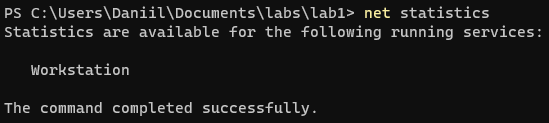
\includegraphics[width=0.9\textwidth]{images/net/statistics.png}
  \caption{Просмотр статистики}
  \label{fig:net-statistics}
\end{figure}

\begin{figure}[H]
  \centering
  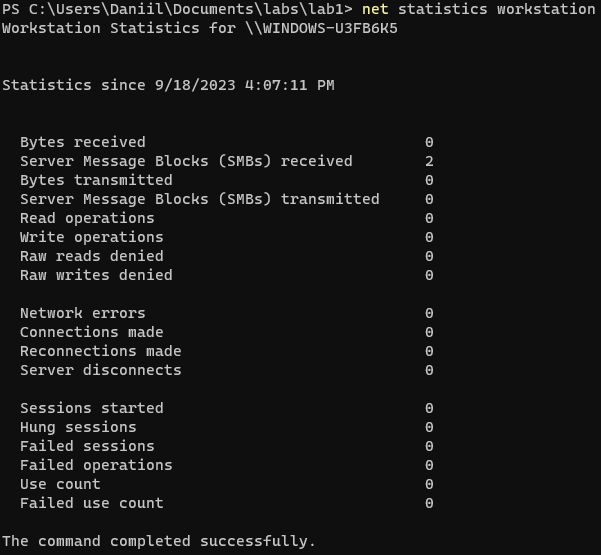
\includegraphics[width=0.9\textwidth]{images/net/statistics-workstation.png}
  \caption{Просмотр статистики рабочей станции}
  \label{fig:net-statistics-workstation}
\end{figure}

Команда \texttt{net localgroup} выводит список групп пользователей для данного
компьютера (см. рис \ref{fig:net-localgroup}). При передаче названия группы в
качестве аргумента выводится информация об этой группе (см. рис.
\ref{fig:net-localgroup-administrators}).

\begin{figure}[H]
  \centering
  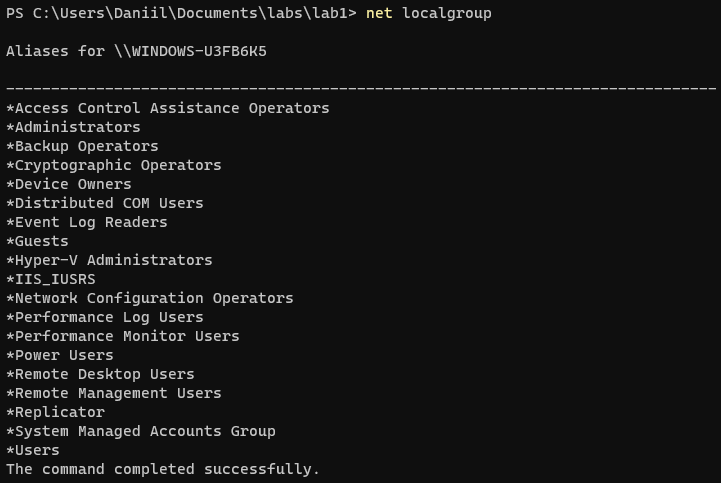
\includegraphics[width=0.9\textwidth]{images/net/localgroup.png}
  \caption{Просмотр списка групп пользователей}
  \label{fig:net-localgroup}
\end{figure}

\begin{figure}[H]
  \centering
  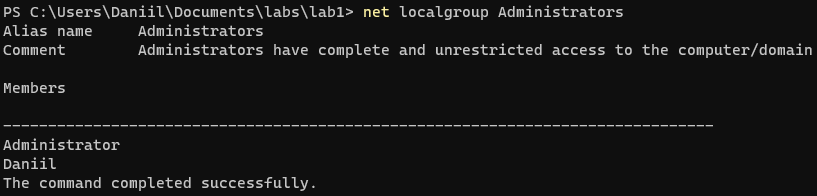
\includegraphics[width=0.9\textwidth]{images/net/localgroup-administrators.png}
  \caption{Просмотр информации о группе Administrators}
  \label{fig:net-localgroup-administrators}
\end{figure}

\subsection{Скрипт для настройки сетевых интерфейсов на Batch}

Исходный код скрипта находится в листинге \ref{code:cmd}. При запуске программы
пользователю предлагается выбрать способ настройки сетевого интерфейса.
Пользователю доступны два способа: с помощью DHCP-сервера или вручную. На рис.
\ref{fig:cmd-dhcp} представлен пример использования программы для получения
всех настроек с помощью DHCP-сервера. На рис. \ref{fig:cmd-static} показан
случай при вводе всех настроек вручную.

\begin{figure}[H]
  \centering
  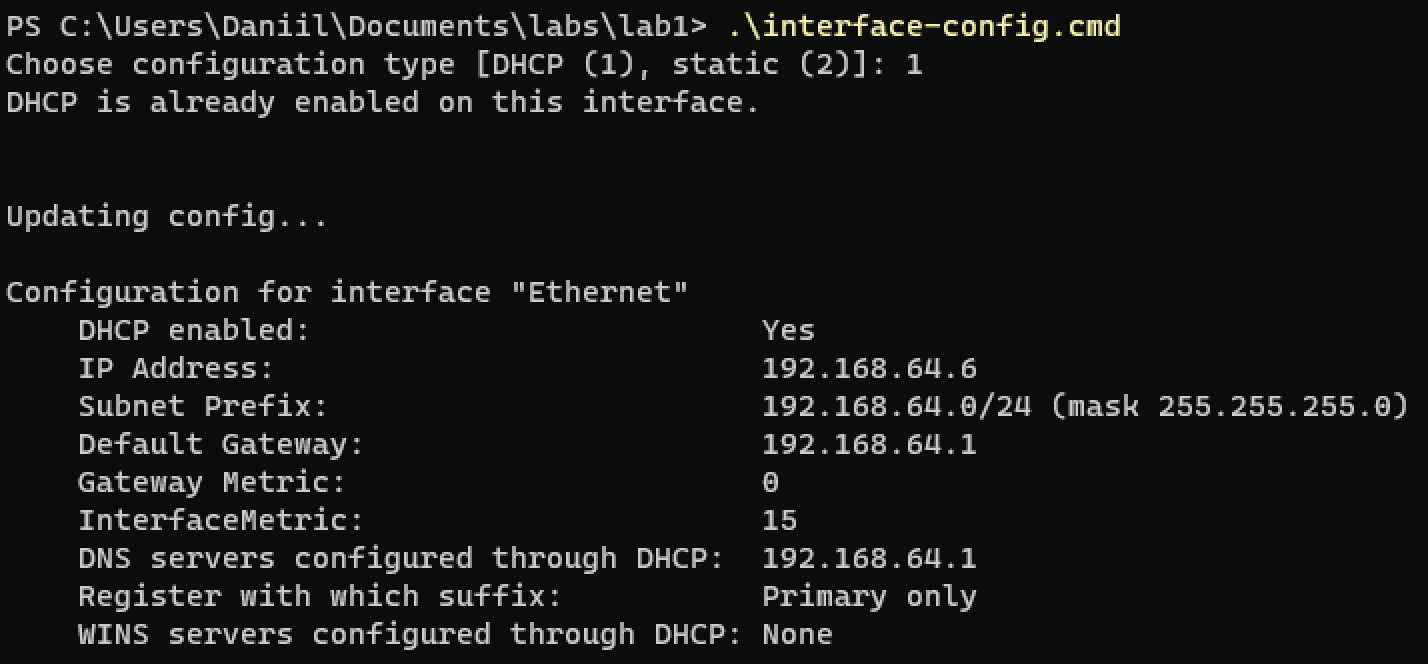
\includegraphics[width=0.9\textwidth]{images/cmd/dhcp.png}
  \caption{Получение всех настроек через DHCP-сервер}
  \label{fig:cmd-dhcp}
\end{figure}

\begin{figure}[H]
  \centering
  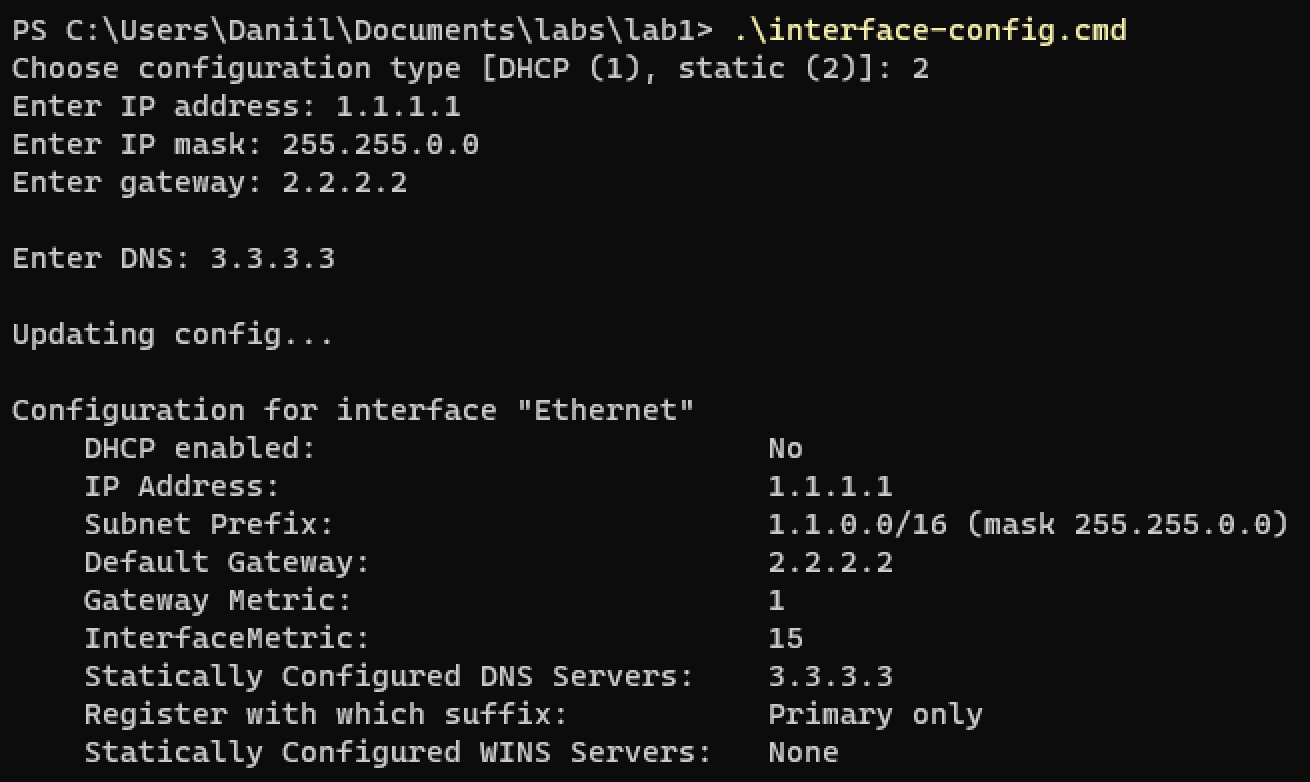
\includegraphics[width=0.9\textwidth]{images/cmd/static.png}
  \caption{Ввод всех настроек вручную}
  \label{fig:cmd-static}
\end{figure}

\subsection{Скрипт для настройки сетевых интерфейсов на PowerShell}

Исходный код скрипта находится в листинге \ref{code:ps1}. Данный скрипт
является расширенной версией предыдущего, в нем появился новый функционал. Для
удобства взаимодействия было добавлено новое меню, в котором пользователь может
\begin{enumerate}
  \item настроить сетевой интерфейс (то же, что делал предыдущий скрипт);
  \item получить модель сетевой карты;
  \item проверить, есть ли физическое подключение;
  \item посмотреть скорость и режим работы адаптера.
\end{enumerate}

На рис. \ref{fig:ps1-dhcp} представлен пример использования программы для
получения всех настроек с помощью DHCP-сервера. На рис. \ref{fig:ps1-static}
показан случай при вводе всех настроек вручную.

\begin{figure}[H]
  \centering
  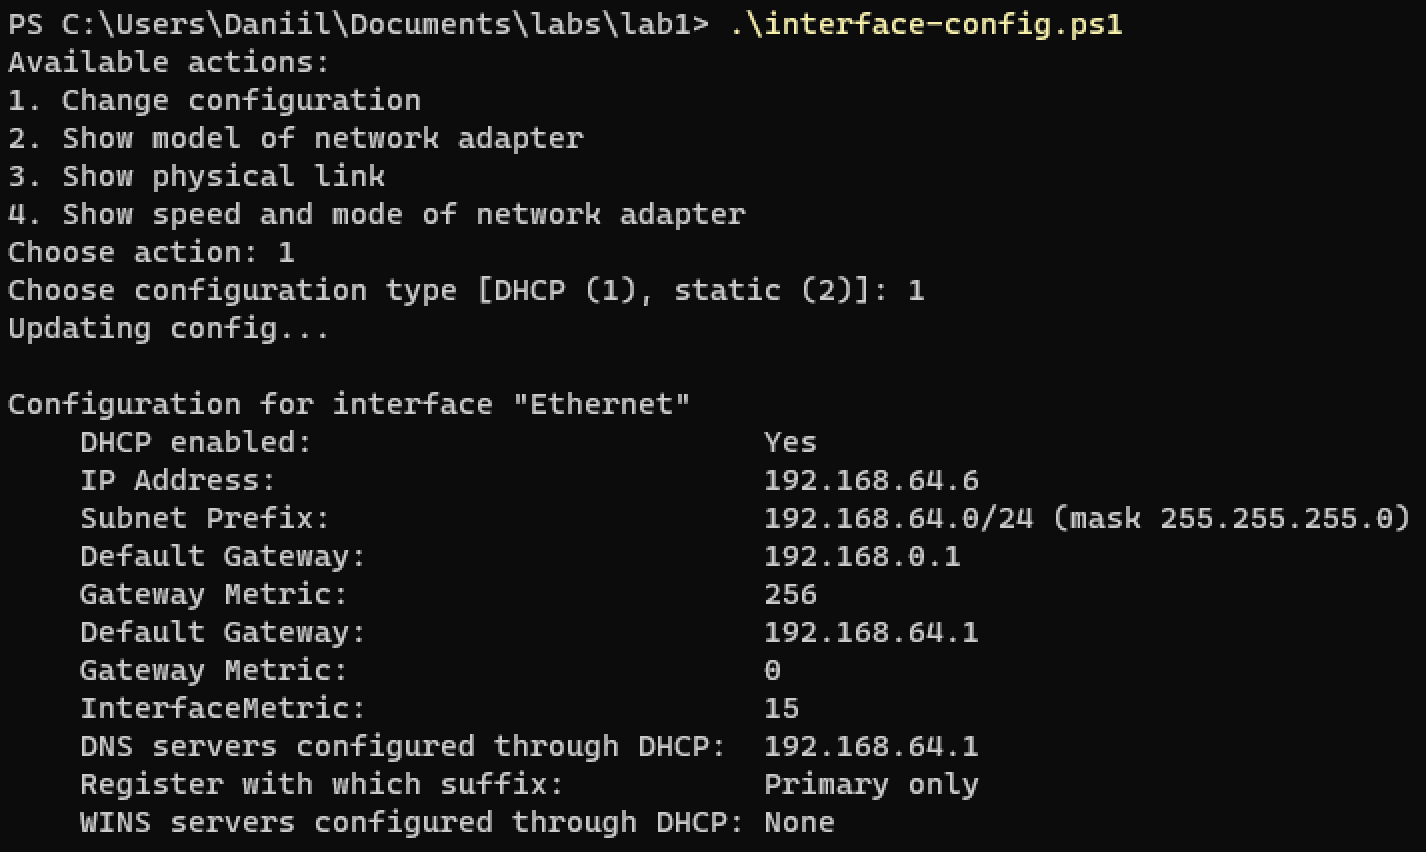
\includegraphics[width=0.9\textwidth]{images/ps1/dhcp.png}
  \caption{Получение всех настроек через DHCP-сервер}
  \label{fig:ps1-dhcp}
\end{figure}

\begin{figure}[H]
  \centering
  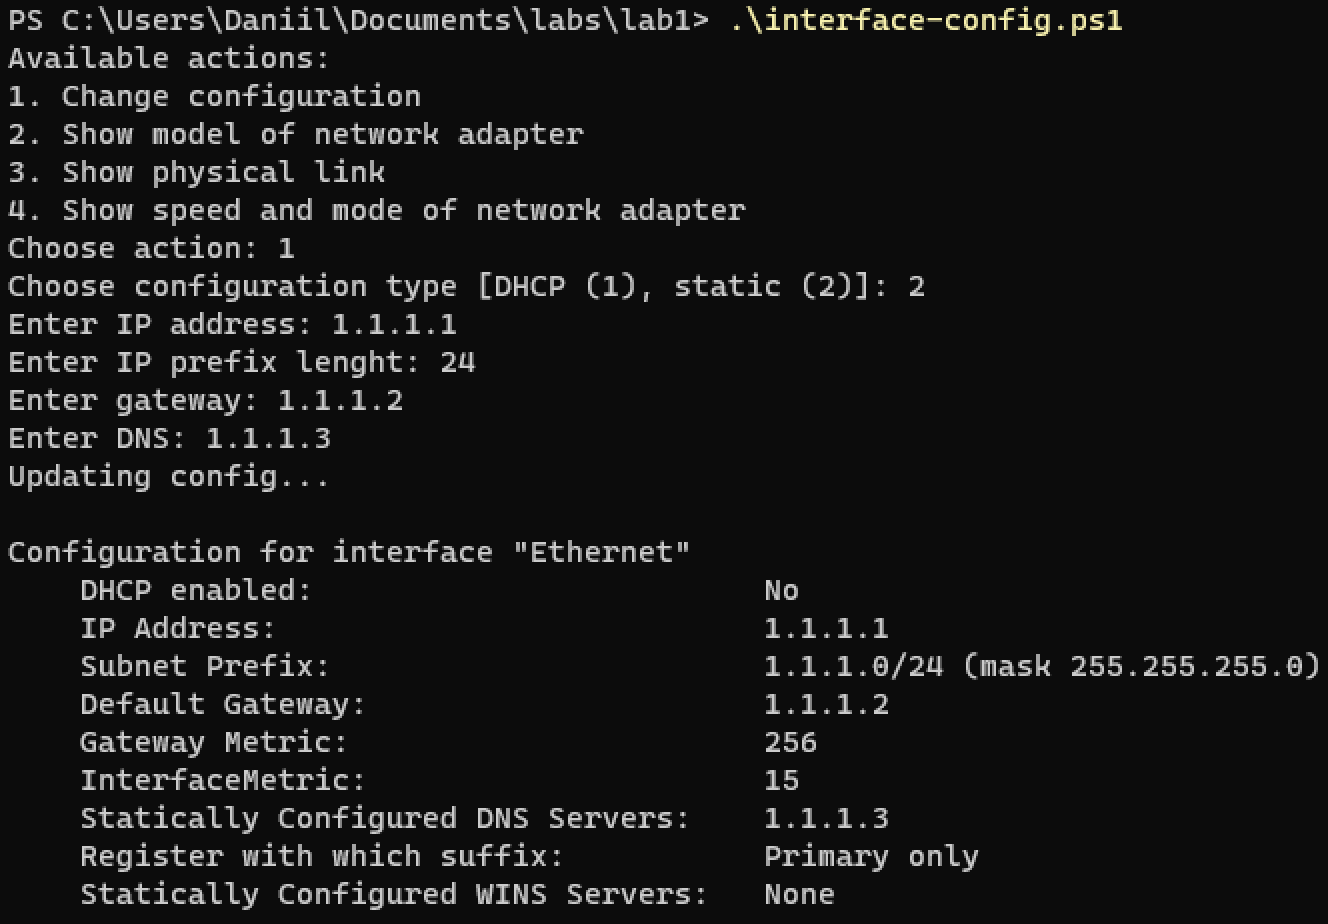
\includegraphics[width=0.9\textwidth]{images/ps1/static.png}
  \caption{Ввод всех настроек вручную}
  \label{fig:ps1-static}
\end{figure}

На рис. \ref{fig:ps1-model} продемонстрировано получение модели сетевой карты.

\begin{figure}[H]
  \centering
  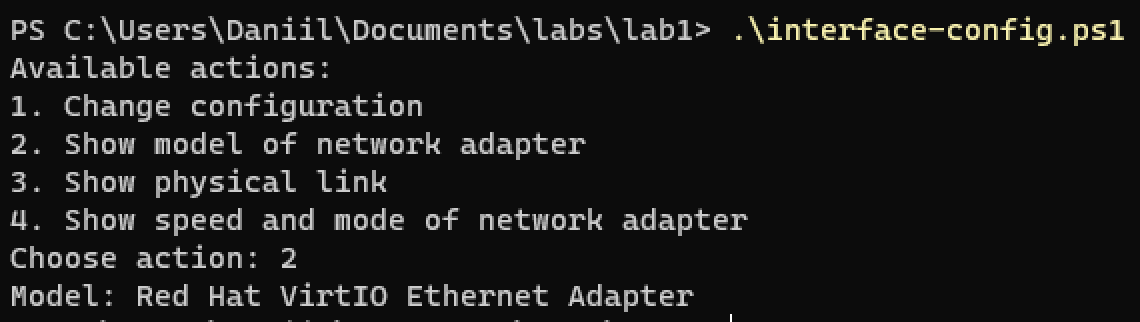
\includegraphics[width=0.9\textwidth]{images/ps1/model.png}
  \caption{Получение модели сетевой карты}
  \label{fig:ps1-model}
\end{figure}

На рис. \ref{fig:ps1-link} показана проверка наличия физического подключения.

\begin{figure}[H]
  \centering
  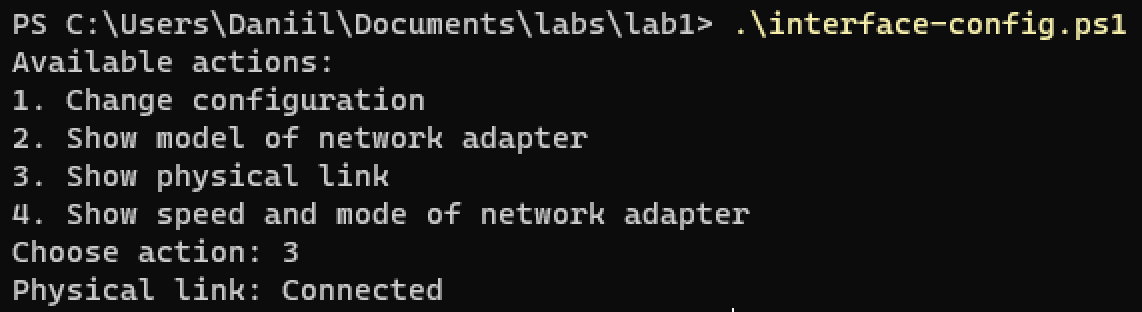
\includegraphics[width=0.9\textwidth]{images/ps1/link.png}
  \caption{Проверка наличия физического подключения}
  \label{fig:ps1-link}
\end{figure}

На рис. \ref{fig:ps1-link} представлен пример получения информации о скорости и
режиме работы адаптера.

\begin{figure}[H]
  \centering
  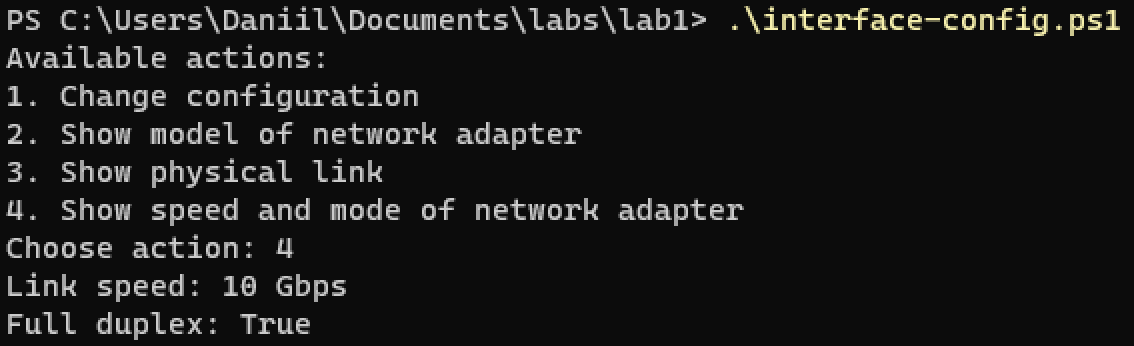
\includegraphics[width=0.9\textwidth]{images/ps1/speed.png}
  \caption{Скорость и режим работы адаптера}
  \label{fig:ps1-speed}
\end{figure}

\newpage

\section{Вопросы и задания}

\begin{enumerate}[leftmargin=*]
  \item Как с помощью командной строки в Windows узнать адрес DNS, на который
  настроен ваш компьютер?

  \textbf{Ответ}:
  \begin{itemize}
    \item с помощью \texttt{ipconfig}: \texttt{ipconfig /all};
    \item с помощью PowerShell: \texttt{Get-DnsClientServerAddress}.
  \end{itemize}
  \item Зачем нужна команда net use? Как с помощью этой утилиты подключить на
  локальный диск R: папку TEST на компьютере SRV (приведите командную
  строку)?

  \textbf{Ответ}: \texttt{net use R: \textbackslash\textbackslash SRV\textbackslash TEST}
  \item Как в Windows из PowerShell переименовать сетевое соединение?

  \textbf{Ответ}: \texttt{Rename-NetAdapter -Name "Ethernet" -NewName "NewEthernet"}
  \item Какие существуют и чем отличаются режимы работы адаптера (duplex)?

  \textbf{Ответ}: существуют следующие режимы работы адаптера:
  \begin{itemize}
    \item симплексный (simplex) — передача осуществляется по линии связи
    только в одном направлении;
    \item полудуплексный (half-duplex) — передача ведется в обоих
    направлениях, но попеременно во времени;
    \item дуплексный (full duplex) — передача ведется одновременно в двух
    направлениях.
  \end{itemize}
\end{enumerate}

\section{Вывод}

В ходе выполнения лабораторной работы я получил практические навыки по
конфигурированию сети в операционных системах Microsoft Windows, ознакомился с
утилитами командной строки, предназначенными для диагностики и настройки сети,
разработал исполняемые файлы, конфигурирующие сетевой интерфейс по заданным
параметрам, ознакомился с форматом записи пути до сетевого ресурса UNC.

\newpage

\section*{Приложение А}

\begin{code}
  \caption{Исходный код программы на Batch}
  \label{code:cmd}
  \inputminted{batch}{../code/interface-config.cmd}
\end{code}

\newpage

\section*{Приложение Б}

\begin{code}
  \caption{Исходный код программы на PowerShell}
  \label{code:ps1}
  \inputminted{powershell}{../code/interface-config.ps1}
\end{code}

\end{document}
